\documentclass[main.tex]{subfiles}

\begin{document}
\chapter{Validation}
\label{chap:validation}
In order to validate the implementation of BFAST and BFAST0n, four datasets were
chosen. Each of the datasets was chosen to test a specific
property of the algorithm. Three of the datasets were
taken from the paper by Verbesselt et al. \cite{bfast} and one from the standard
dataset library for the R programming language \cite{r-datasets}. The results were compared to
the same data applied to the original R-implementation of BFAST and BFAST0n
\cite{bfast-github}. Both mine and R implementation find exactly same
breakpoints for the same input and parameter values. There are however some
small differences in the decomposition due to different implementations of STL
and linear regression. Chapter \ref{chap:implementation} elaborates on both of
these points. This chapter only covers the validation of the BFAST algorithm,
but the BFAST0n implementation was tested in a similar manner.

\section{\texttt{nile}}
\label{sec:val_nile}
Measurements of the annual flow of the river Nile at Aswan 
1871–1970. With apparent breakpoint near 1898 when the first Ashwan dam was built
From \cite{r-datasets}. There is
no seasonal component, since there is only a single observation each year. This
tests the breakpoint estimating capacity without STL and seasonal model.
Following parameter values were used:
\begin{itemize}
\item \texttt{season}= "none"
\item $\alpha = 0.05$
\item $h = 0.15$
\end{itemize}
The results can be seen on Figure \ref{plt:nile}.
\begin{figure}
  \centering
  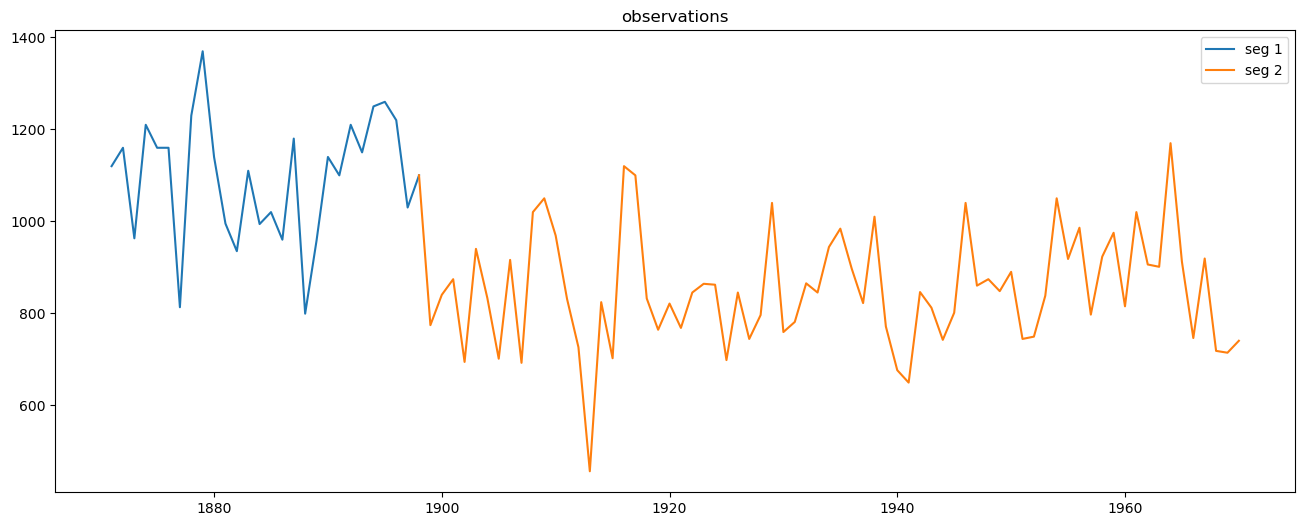
\includegraphics[width=\textwidth]{imgs/nile.png}
  \caption{Result of applying BFAST to the \texttt{nile} dataset.
    \texttt{season} = ``none'' had been chosen, hence no decomposition was done}
  \label{plt:nile}
\end{figure}

\section{\texttt{harvest}}
\label{sec:val_harvest}
16-day NDVI Time Series for a Pinus Radiata Plantation, with approximately 23
observation per year from \cite{bfast}. There are 4 breakpoints in the trend
component exclusively. The results can be seen on Figure \ref{plt:harvest}.
Following parameter values were used:
\begin{itemize}
\item \texttt{season}= ``harmonic''
\item $\alpha = 0.05$
\item $h = 0.15$
\end{itemize}

\begin{figure}
  \centering
  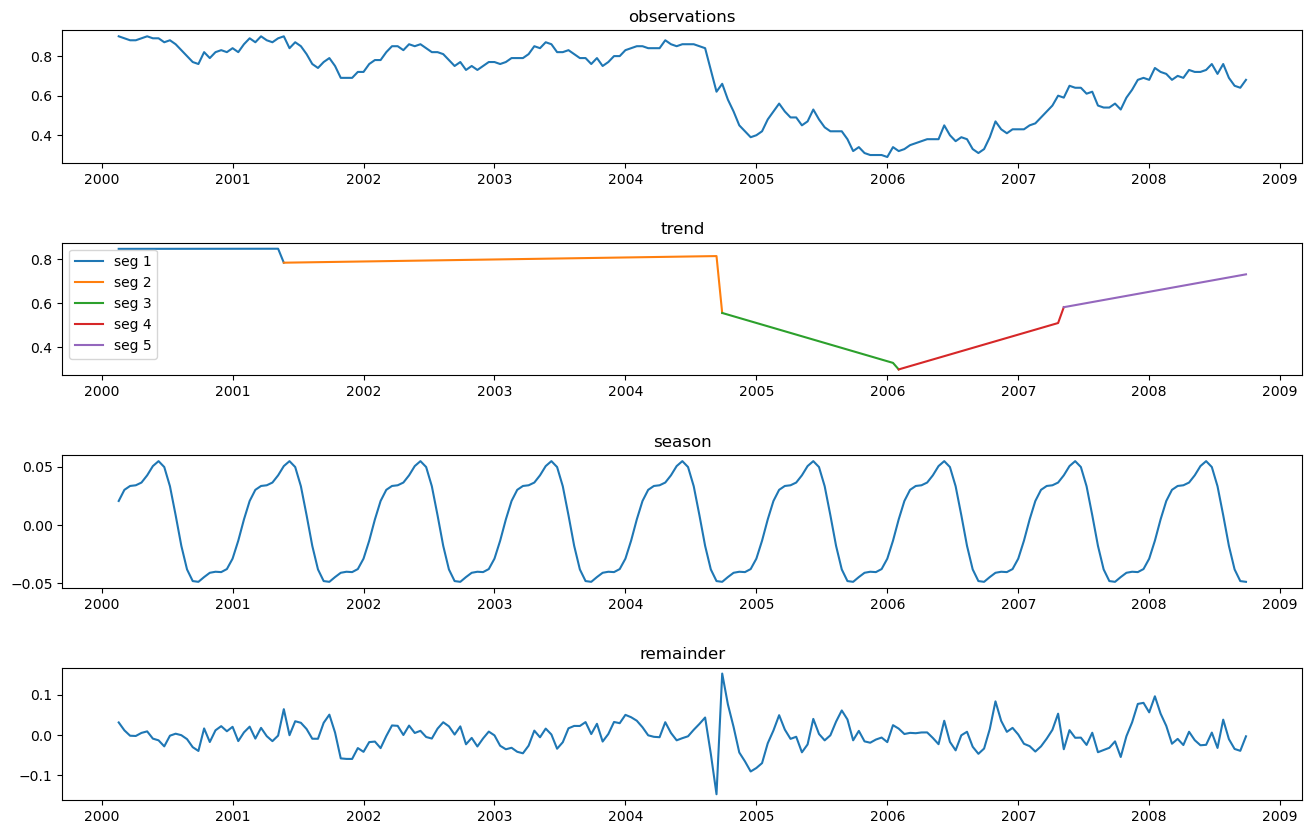
\includegraphics[width=\textwidth]{imgs/harvest.png}
  \caption{Result of applying BFAST to the \texttt{harvest} dataset}
  \label{plt:harvest}
\end{figure}

\section{\texttt{simts}}
\label{sec:val_simts}
Simulated seasonal 16-day NDVI time series from \cite{bfast}. The seasonal
component has a single breakpoint that is difficult to detect. Hence, following
parameter values were used:
\begin{itemize}
\item \texttt{season}= "harmonic"
\item $\alpha = 0.35$
\item $h = 0.3$
\item \texttt{max\_iter} = 2
\end{itemize}
The results can be seen on Figure \ref{plt:simts}.

\begin{figure}
  \centering
  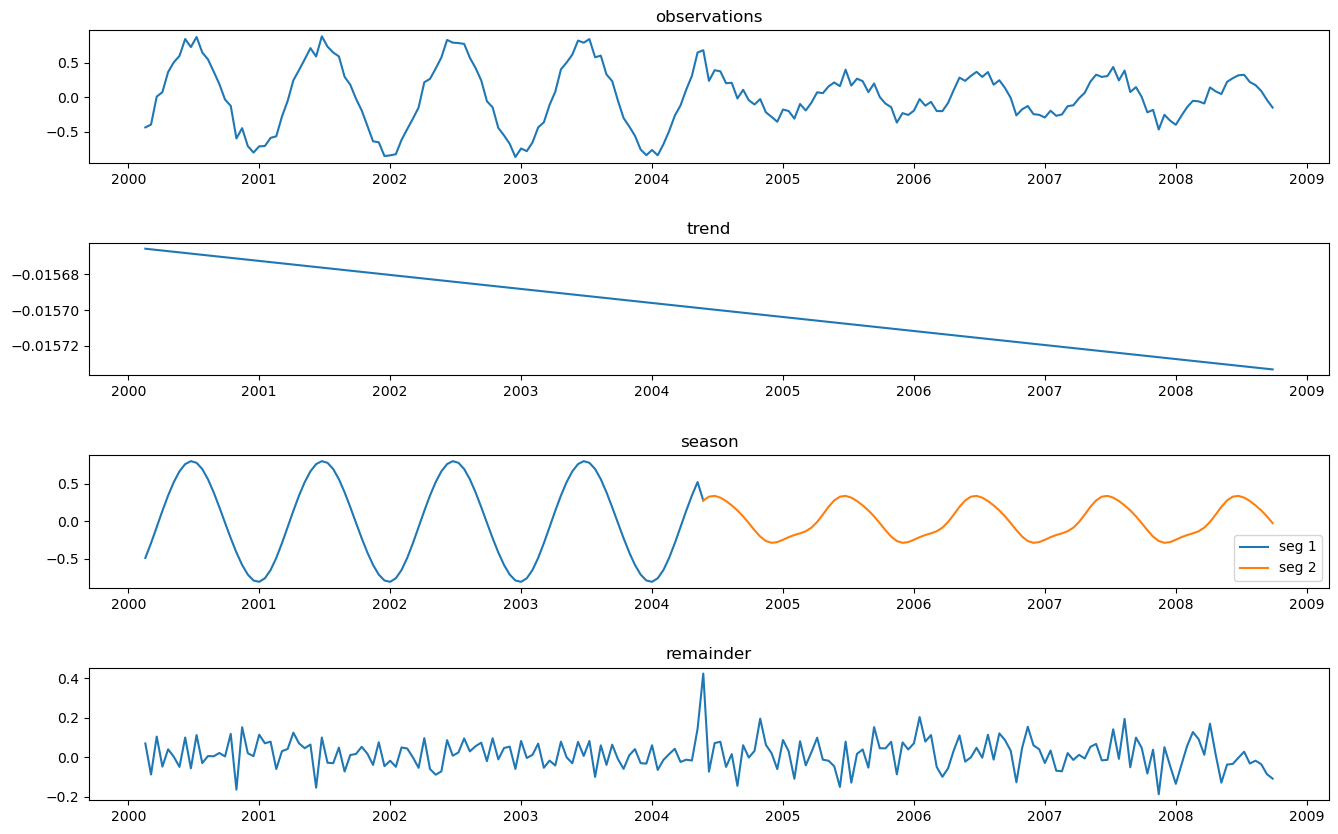
\includegraphics[width=\textwidth]{imgs/simts.png}
  \caption{Result of applying BFAST to the \texttt{simts} dataset}
  \label{plt:simts}
\end{figure}

\section{\texttt{ndvi}}
\label{sec:val_ndvi}
A random NDVI time series with missing values. BFAST should pass the missing
values into the seasonal, trend and remainder components, and my implementation
accomplishes that. Frequency is set to 24.
There is a single breakpoint in the trend component.
Source: \cite{bfast}. Following parameter values were used:
\begin{itemize}
\item \texttt{season}= ``dummy''
\item $\alpha = 0.05$
\item $h = 0.15$
\end{itemize}
The results can be seen on Figure \ref{plt:ndvi}.
\begin{figure}
  \centering
  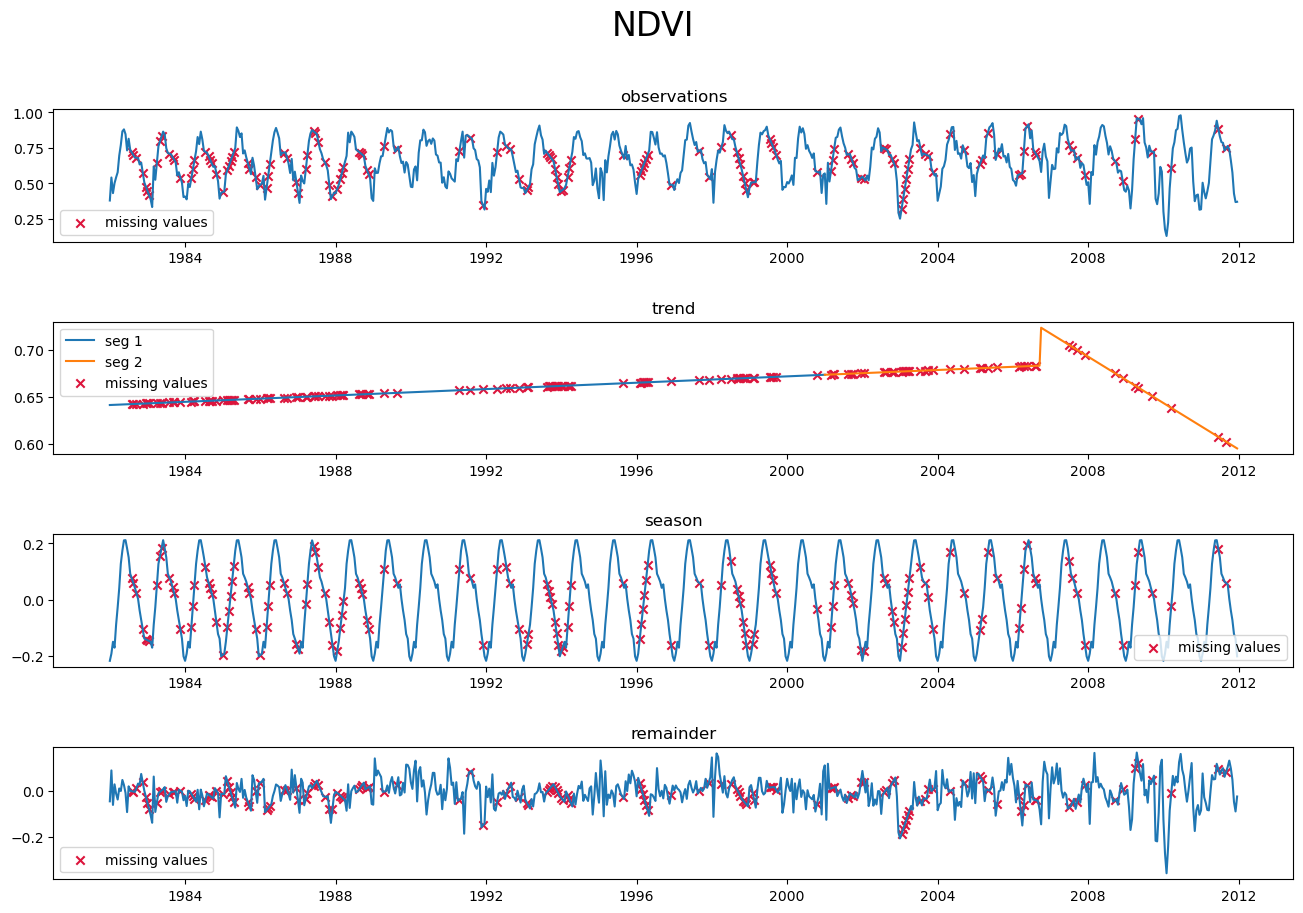
\includegraphics[width=\textwidth]{imgs/ndvi.png}
  \caption{Result of applying BFAST to the \texttt{NDVI} dataset. Red crosses
    denote the missing values in the original time series}
  \label{plt:ndvi}
\end{figure}


\biblio
\end{document}
